% Remember to input this to the presentative tex file before compiling.
\section{Basics}
\subsection{Typesetting and Math}
\begin{frame}{Typesetting and Math}
Commands can be used with the backlash \textbackslash. \\
To get a new line, we need to use two backlashes \textbackslash\textbackslash \\

\end{frame}

\begin{frame}[fragile]
Some generally useful commands:
\begin{verbatim}
    \textbf{text} % Bolding Text
    \textit{text} % Italicised Text
    \textcolor{color}{text} % Coloured Text
    \href{link}{name of link} % Create Hyperlinks
\end{verbatim}
\end{frame}

\begin{frame}[fragile]
We can create unordered list by using itemize:
\begin{itemize}
    \item First Ele
    \item Second Ele
    \item Third Ele
\end{itemize}
\begin{verbatim}
\begin{itemize}
    \item First Ele
    \item Second Ele
    \item Third Ele
\end{itemize}
\end{verbatim}

or we can create ordered list using enumerate:
\begin{enumerate}
    \item First Ele
    \item Second Ele
    \item Third Ele
\end{enumerate}

\begin{verbatim}
\begin{enumerate}
    \item First Ele
    \item Second Ele
    \item Third Ele
\end{enumerate}
\end{verbatim}

\end{frame}

\begin{frame}[fragile]

Examples of mathematical symbols
\begin{verbatim}
    $\pi, \alpha \log(\beta)$ 
\end{verbatim}

will yield: $\pi, \alpha \log(\beta)$ 

\end{frame}

\begin{frame}[fragile]
For inline equations, like $a^2 + b^2 + c^2$, we use one \$:
\begin{verbatim}
    $a^2 + b^2 + c^2$
\end{verbatim}

For equations that span a few lines, we use align (there are multiple ways but this way is the most general way): 
\begin{verbatim}
\begin{align*}
    \frac{r^{3}}{T^{2}} &= \frac{GM}{4\pi^2} \\
    a^2 + b^2 &= c^2 \\
    F_g &= \frac{GM}{r^2}
\end{align*}  
\end{verbatim}
will create the following:
\begin{align*}
    \frac{r^{3}}{T^{2}} &= \frac{GM}{4\pi^2} \\
    a^2 + b^2 &= c^2 \\
    F_g &= \frac{GM}{r^2}
\end{align*}  
\\
Note the use of \textbackslash\textbackslash  to get a new line.
We use \& to ensure the equations line up at the equals sign

\end{frame}

\newcommand{\pyth}[3]{$#1 + #2 + #3$}

\begin{frame}[fragile]
To define custom equations, define them at the top of the page like so:

\begin{verbatim}
    \newcommand{\name_of_command}[number_of_variables]{custom_command}
    \newcommand{\pyth}[3]{$#1 + #2 + #3$}
\end{verbatim}

We can then call these commands by writing
\begin{verbatim}
    \pyth{a}{b}{c}
\end{verbatim}
which outputs \pyth{a}{b}{c}

\end{frame}

\newcommand{\abundance}[2]{$\Big[\frac{#1}{#2}\Big]$}

\begin{frame}[fragile]
Task: 
\begin{enumerate}
    \item Recreate the following equation:
    \begin{align*}
        M_\odot = 1.99 \times 10^{30} kg \\
        \gamma = \frac{1}{\sqrt{1 - \frac{v^2}{c^2}}} \\
        B_\nu = \frac{2h \nu^3}{c^2} \frac{1}{\exp(h \nu /kT) - 1}
    \end{align*}
    \item Define a custom command that automatically gives you the relative abundance between two elements:
    \begin{verbatim}
        \abundance{Fe}{H}
        \abundance{C}{N}
    \end{verbatim}
    should output \abundance{Fe}{H} and \abundance{C}{N}
    \item List out steps to your daily commute using an ordered list
\end{enumerate}
\end{frame}


\begin{frame}[fragile]
Solution: 
\begin{enumerate}
    \item Recreate the following equation:
    \begin{verbatim}
        
        M_\odot = 1.99 \times 10^{30} kg \\
        \gamma = \frac{1}{\sqrt{1 - \frac{v^2}{c^2}}} \\
        B_\nu = \frac{2h \nu^3}{c^2} \frac{1}{\exp(h \nu /kT) - 1}
    \end{verbatim}
    \item Define a custom command that differentiates a variable for you:
    \begin{verbatim}
        \newcommand{\abundance}[2]{$\Big[\frac{#1}{#2}\Big]$}
    \end{verbatim}
    \item Daily Commute
    \begin{verbatim}
        \begin{enumerate}
            \item Don't have coffee
            \item Ded
        \end{enumerate}
    \end{verbatim}
\end{enumerate}
\end{frame}

\subsection{Figures}

\begin{frame}{Figure Example}

\begin{figure}
    \centering
    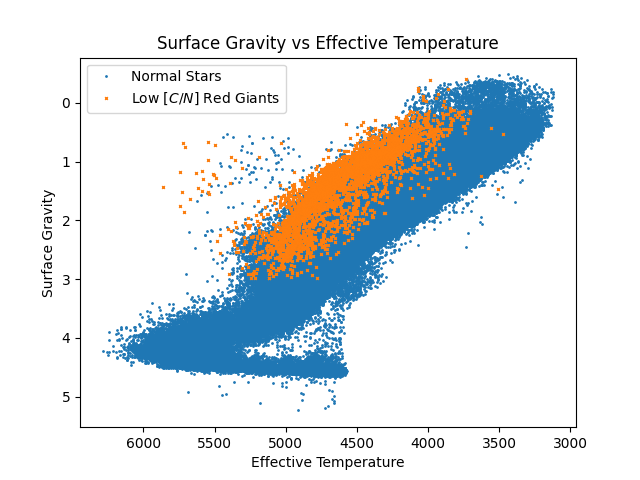
\includegraphics[width=\columnwidth/3]{Figures/AGBProof.png}
    \caption{Verifying whether low \CN stars are AGB stars. Orange data points are for low \CN red giants while the blue data points consist of all the stars in the APOGEE data set. The orange spots that are above the main group of stars are potential AGB stars.}
    \label{fig:AGB_PROOF}
\end{figure}

FYI: the label command can be used just to mark some arbitrary place (e.g. you can label a section or a paragraph if you want to cite them later).
\end{frame}

\begin{frame}[fragile]

Structure of a figure
\begin{verbatim}
\begin{figure}
    \centering
    \includegraphics[additional commands]{location of figure}
    \caption{random text}
    \label{label can be used to reference image}
\end{figure}
\end{verbatim}

The figure on the previous slide uses:

\begin{verbatim}
\begin{figure}
    \centering
    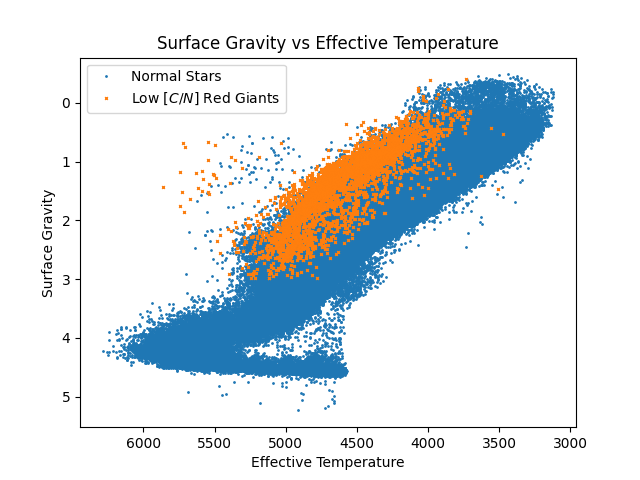
\includegraphics[width=\columnwidth/3]{Figures/AGBProof.png}
    \caption{Verifying whether low \CN stars are AGB stars...}
    \label{fig:AGB_PROOF}
\end{figure}
\end{verbatim}

We can reference the figure \ref{fig:AGB_PROOF} now that its labeled using:
\begin{verbatim}
    \ref{fig:AGB_PROOF}
\end{verbatim}

    
\end{frame}

\begin{frame}

Task:
\begin{itemize}
    \item Include JWST image 
    \begin{itemize}
        \item Make sure it fits
        \item Include a caption
        \item Label it something sensible and reference it
    \end{itemize}
\end{itemize}
    
\end{frame}

\begin{frame}[fragile]
Solution:
\begin{verbatim}
\begin{figure}
    \centering
    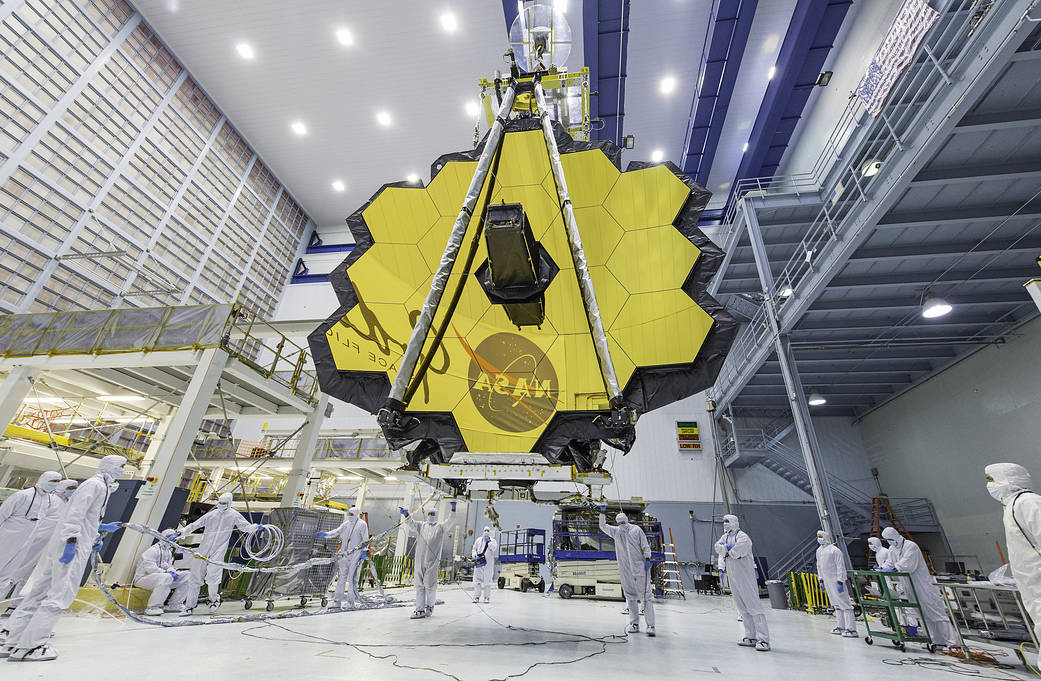
\includegraphics[width=\columnwidth]{photos/jwst.jpg}
    \caption{coolio spaghettio}
    \label{jswt}
\end{figure}

Figure \ref{jswt}
\end{verbatim}

\end{frame}

\subsection{Bibliograph}

\begin{frame}[fragile]
In your research folder, there should be a .bib files where you put your bibliography.
\begin{itemize}
    \item When you cite any of the articles in your .bib file, it should automatically be included in your citations at the bottom of your document
    \item To cite any article, simply write (there should be some citations you can use in the template)
    \begin{verbatim}
        \cite{citation}
        \cite{Martell02}
    \end{verbatim}
\end{itemize}

\end{frame}


\begin{frame}[fragile]
To add another citation, simply export citation from your source of choice and add to the .bib file. \\
Make sure that it is in the form BibTeX. \\
It should look something like this (
P.S. you can change the 2023MNRAS.523LL..80B part (this is an alias, so we can change it to make it easier to recognise, e.g. Kirsten23)
P.S.S your articles maybe different as there are many more fields
\begin{verbatim}
    @ARTICLE{2023MNRAS.523L..80B,
       author = {{Banks}, Kirsten A. and {Ho}, ...}
        title = "{CN and CO features: ...}",
      journal = {\mnras},
     keywords = {asteroseismology, stars: evolution, ...},
     ...
}
\end{verbatim}
\end{frame}


\begin{frame}[fragile]
Task:
\begin{itemize}
    \item Find a new citation of ADS and add it to your document
    \item Cite it and find it in your bottom of your compiled PDF
\end{itemize}
\end{frame}

